\documentclass[11pt]{article}

\usepackage[review]{acl}
\usepackage{times}
\usepackage{latexsym}
\usepackage[T1]{fontenc}
\usepackage[utf8]{inputenc}
\usepackage{microtype}
\usepackage{inconsolata}
\usepackage{amsmath,amssymb}
\usepackage{booktabs}
\usepackage{graphicx}
\usepackage{multirow}
\usepackage{etoolbox}

\title{Trace-Source Mismatch Drives Dose-Dependent Erosion of Step Dependence Under Reasoning SFT}

\author{Anonymous EACL 2027 SRW Submission}

\begin{document}
\maketitle

\begin{abstract}
Supervised fine-tuning (SFT) on chain-of-thought (CoT) traces can degrade whether a language model's final answer causally depends on its intermediate steps.
We test what drives this degradation on Qwen3-8B (4-bit LoRA) using deterministic intermediate-value interventions and pre-registered protocols across GSM8K and GSM-Plus.
First, while counterfactual trace augmentation improves exact step-following over plain SFT on the sealed GSM8K test (+4.8 pp, $p=0.0018$), the gain does not replicate under numerical substitution on GSM-Plus (+1.5 pp, $p=0.689$; holdout +1.4 pp, $p=0.512$), whereas plain SFT's drop below the untuned base model does replicate ($-9.2$ pp, $p=0.0076$).
Second, isolating trace source on identical questions, fine-tuning on self-generated traces preserves step dependence over human-written traces across two seeds and two disjoint 500-item GSM-Plus splits (+8.6 to +14.3 pp, all $p \le 0.023$).
Third, a pre-registered 5-level nested mixing sweep (0/25/50/75/100\% human traces, 2 seeds, 10 adapters) confirms a dose-dependent erosion at the adapter level ($b_{\text{human}} = -0.649$, $t(7) = -5.38$, $p = 0.0010$), persisting on the 59-question common intersection ($p = 0.0034$) and on originally correct items ($p = 0.0475$).
A post-hoc continuation audit reveals a sharp mechanism: 94\%--97\% of continuations still causally plug the edited number into \texttt{Calc:}, step bypass stays flat ($p = 0.335$), and 80\% of the \texttt{follows} drop stems from downstream trajectory derailment \emph{after} consuming the edit ($p = 0.0014$).
\end{abstract}

\section{Introduction}
\label{sec:intro}

Language models often produce plausible chain-of-thought (CoT) rationales whose intermediate steps do not causally govern the final answer \citep{lanham2023measuring,turpin2024language}.
Recent work shows that ordinary supervised fine-tuning (SFT) can \emph{lower} CoT faithfulness relative to the untuned base model \citep{lobo2024impact}, prompting training-time remedies such as counterfactual trace augmentation and intervention-based objectives \citep{paul2024frodo,swaroop2025lift,akter2025ccr,wang2026case}.
Yet a basic diagnostic question remains under-explored: \emph{which property of reasoning SFT causes step dependence to erode in the first place?}

Parallel work on post-training distribution shift shows that off-policy SFT on unfamiliar or externally authored demonstrations induces hallucinations, forgetting, and train--inference mismatch compared to on-policy or self-generated trajectories \citep{gekhman2024does,shenfeld2026sdft,zhang2026onpolicysft,zhao2026onpolicyefficient}.
Those studies evaluate accuracy, factual forgetting, or token efficiency, not causal dependence on intermediate reasoning steps.

We bridge these two lines through pre-registered, deterministic intervention studies on Qwen3-8B (4-bit LoRA) over GSM8K \citep{cobbe2021training} and GSM-Plus \citep{li2024gsmplus}.
Instead of LLM judges, we enforce an auditable \texttt{Step}/\texttt{Calc} format inside \texttt{<think>} blocks, perturb one intermediate arithmetic result, and test whether the continuation's final answer matches the analytically propagated target (\texttt{follows}):
\begin{enumerate}
    \setlength{\itemsep}{1pt}
    \item \textbf{CF SFT is distribution-bound (H1/H2):} Counterfactual SFT beats plain SFT on the sealed GSM8K test (+4.8 pp, $p=0.0018$), but fails across two GSM-Plus splits (+1.5 and +1.4 pp, $p \ge 0.51$), whereas plain SFT's drop below base replicates ($-9.2$ pp, $p=0.0076$).
    \item \textbf{Trace source drives the gap (H3):} On 229 length- and format-matched problems, self-generated traces beat human-written traces across two seeds and two disjoint 500-item GSM-Plus splits (+8.6 to +14.3 pp, all $p \le 0.023$).
    \item \textbf{Dose-dependent erosion \& mechanism (H4):} Across nested 0/25/50/75/100\% human-trace mixes (10 adapters), human-trace fraction erodes \texttt{follows} ($b_{\text{human}} = -0.649$, $p = 0.0010$) while lowering accuracy by $\sim$9 pp at matched format validity. Post-hoc decomposition shows 80\% of this drop is downstream derailment \emph{after} consuming the edit ($p=0.0014$), not step bypass ($p=0.335$).
\end{enumerate}

\section{Related Work}
\label{sec:related}

\paragraph{CoT Faithfulness and Counterfactual SFT.}
\citet{lanham2023measuring} and \citet{turpin2024language} show that CoT explanations frequently act as post-hoc rationalizations.
\citet{lobo2024impact} find that QLoRA SFT on GSM8K reduces faithfulness relative to the base model, while \citet{han2026rfeval} compare large-scale SFT and RL stages via LLM-judged counterfactual edits.
To improve faithfulness, \textsc{Frodo} \citep{paul2024frodo}, \textsc{LIFT} \citep{swaroop2025lift}, CCR \citep{akter2025ccr}, CST \citep{hase2026cst}, \textsc{CASE} \citep{wang2026case}, and Chain of Faith \citep{meng2026chainoffaith} introduce counterfactual preference, likelihood, masking, or RL rewards.
We complement these methods by isolating whether \emph{trace-source mismatch} in standard SFT causes the underlying drop.

\paragraph{Off-Policy vs.\ On-Policy SFT.}
\citet{gekhman2024does} show that fine-tuning on unfamiliar factual knowledge linearly increases hallucination.
Recent work mitigates off-policy distribution mismatch via self-distillation \citep{shenfeld2026sdft}, distribution-discriminant on-policy SFT \citep{zhang2026onpolicysft}, and filtered self-generated rollouts \citep{zhao2026onpolicyefficient}, focusing on accuracy, continual learning, or brevity.
\citet{peng2026posthoc} study post-hoc rationalization from answer-visible reverse CoT generation; in contrast, all traces in our study are valid forward solutions.
Most closely related methodologically, \citet{xu2026evidencebypass} show that on-policy distillation can \emph{increase} bypass of edited \emph{external documents} in scientific QA---a valuable contrast to our finding that self-generated SFT \emph{preserves} reliance on \emph{internal arithmetic steps} (Section~\ref{sec:discussion}).

\section{Method and Pre-Registered Protocols}
\label{sec:method}

\paragraph{Structured Format and Deterministic Intervention.}
We train Qwen3-8B (4-bit MLX quantization) with LoRA (rank 8, scale 20, 8 target layers, lr $5\times 10^{-5}$, batch size 1, max sequence length 512) to emit explicit \texttt{Step}/\texttt{Calc} pairs inside \texttt{<think>} tags followed by \mbox{\texttt{Answer: <value>}}.
Given a generated trace, our deterministic planner identifies an intermediate \texttt{Calc} expression whose result is reused downstream, replaces that numeric result with a perturbed value, truncates the trace immediately after the edited line, and continues greedy decoding (max 512 tokens).
Each continuation is classified deterministically into \texttt{follows} (exact match to the analytically propagated answer), \texttt{follows\_rounded}, \texttt{follows\_approximate}, \texttt{reverted} (returns to the original unperturbed answer), \texttt{moved} (changes answer when the original trace had no valid analytic target, \texttt{expected = None}), \texttt{other}, or \texttt{no\_answer}.
Following correctness-conditioning critiques, primary analyses include \emph{all} eligible traces regardless of whether the original answer was correct; originally correct items are reported as a sensitivity check.
Figure~\ref{fig:example} illustrates the format and a single-step edit.

\begin{figure}[t]
\centering
\scriptsize
\fbox{\parbox{0.94\columnwidth}{\ttfamily
\textbf{Original:} Step 1: Clips in May. Calc: 48/2=24 \\
Step 2: Total clips. Calc: 48+24=72 $\rightarrow$ Answer: 72\\[2pt]
\textbf{Edit (prefix):} Step 1: Clips in May. Calc: 48/2=\textbf{30}\\
\textbf{Target:} 48+30=\textbf{78} \hfill (\texttt{follows}: 78;\ \texttt{reverted}: 72)
}}
\caption{Illustration of the \texttt{Step}/\texttt{Calc} format and a deterministic intermediate perturbation.}
\label{fig:example}
\end{figure}

\paragraph{Experiments and Pre-Registration.}
All four hypotheses (H1--H4) were pre-registered via git commits before evaluating target splits:
\begin{itemize}
    \setlength{\itemsep}{1pt}
    \item \textbf{H1 \& H2 (CF vs.\ Plain vs.\ Base):} 2,000-step adapters on enriched GSM8K plain (7,061 items) vs.\ plain+CF traces (10,180 items), tested once on sealed GSM8K (1,319 items) and replicated on GSM-Plus numerical substitutions (500-item split + 819-item holdout). Untuned \texttt{base\_prefill} uses format instructions and a \texttt{Step 1:} prefill.
    \item \textbf{H3 (Self vs.\ Human):} From 400 GSM8K train problems, we keep all 229 \texttt{base\_prefill} traces passing format, arithmetic, and answer checks (\texttt{self}), paired with the same 229 human GSM8K traces in \texttt{Step}/\texttt{Calc} (\texttt{human}; 0 off-format, 0 rows $>512$ tokens, mean 209.4 vs.\ 210.2 tokens; 200 steps, seeds 0/1), evaluated on 500 GSM-Plus items.
    \item \textbf{H4 (Dose Sweep):} Via SHA-256 ranking on the 229 items, we build nested sets $S_0 \subset S_{25} \subset S_{50} \subset S_{75} \subset S_{100}$ (0/57/114/172/229 human rows, exact row order preserved). Reusing the 4 H3 endpoint adapters and training 6 interior adapters (25/50/75\%, seeds 0/1), we evaluate all 10 on 500 disjoint GSM-Plus holdout items.
\end{itemize}

\paragraph{Adapter-Level Primary Test (H4 Amendment).}
Prior to running analysis on H4, we amended the primary test to address adapter-level pseudo-replication: a question-only random-intercept GLMM treats observations within an adapter as independent, inflating Type-I error if adapter training variance $\tau > 0$.
Our pre-registered primary test instead computes the empirical logit $y_c = \operatorname{logit}\big((f_c + 0.5)/(n_c + 1)\big)$ for each of the $10$ adapter cells $c=(\text{seed}, \text{ratio})$ and fits OLS $y_c = b_0 + b_{\text{human}} x_c + b_{\text{seed}} s_c$ with a two-sided $t$-test ($\text{df}=7$, $\alpha=0.05$) on $x_c = k/229$.
Because original traces with flagged arithmetic (\texttt{expected = None}) can never be labeled \texttt{follows}, our primary metric (\textbf{B1}) restricts to planned items with \texttt{expected != None} and reports the flagged-trace rate separately; the original all-planned metric is reported as a secondary test.
Per our pre-registered wording rule, we claim ``monotonic'' erosion only if H4 is significant \emph{and} the 5-level mean logits strictly decrease across all intermediate ratios.

\begin{figure*}[t]
\centering
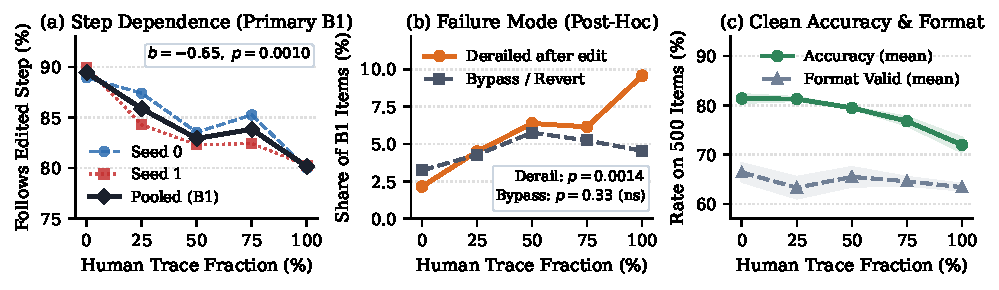
\includegraphics[width=\textwidth]{fig_dose_response.pdf}
\caption{H4 dose-response on 500 clean GSM-Plus holdout items across 10 adapters (5 nested human-trace ratios $\times$ 2 seeds). \textbf{(a)} Pre-registered primary B1 step-following rate declines with human-trace fraction ($p=0.0010$). \textbf{(b)} Post-hoc decomposition: step bypass/reversion stays flat ($p=0.335$), whereas downstream derailment \emph{after} plugging the edited value into \texttt{Calc:} surges $>4\times$ ($2.2\% \rightarrow 9.6\%$, $p=0.0014$). \textbf{(c)} Format validity stays matched while mean accuracy drops from 81.4\% to 72.0\%.}
\label{fig:dose}
\end{figure*}

\section{Results}
\label{sec:results}

\subsection{H1--H3: CF Fails on GSM-Plus; Trace Source Replicates}

Table~\ref{tab:h1_h3} summarizes the paired McNemar tests across H1--H3.
On the sealed GSM8K test, counterfactual SFT (\texttt{CF}) follows edited steps more often than plain SFT (+4.8 pp, $p=0.0018$), replicating \citet{swaroop2025lift}, though both trail \texttt{base\_prefill} in accuracy (79.8\% and 78.8\% vs.\ 88.5\%).
A post-hoc comparison on GSM8K suggested plain SFT drops below \texttt{base\_prefill} (78.5\% vs.\ 85.3\%, $p=0.0003$).
On GSM-Plus numerical substitutions, this plain-SFT drop replicates under pre-registration (\textbf{H2}: $-9.2$ pp, $p=0.0076$, Holm-adjusted $\alpha=0.025$), whereas \textbf{H1} (\texttt{CF} vs.\ \texttt{Plain}) vanishes across both the 500-item split (+1.5 pp, $p=0.689$) and the 819-item holdout (+1.4 pp, $p=0.512$, 70\% power for the GSM8K effect size).

In stark contrast, \textbf{H3} (\texttt{self} vs.\ \texttt{human}) produces a large, replicable gap on GSM-Plus: +8.6 pp on Seed 0 ($p=0.023$) and +9.7 pp on Seed 1 ($p=0.007$), and replicates again on the disjoint 500-item H4 holdout (+14.3 pp, $p=1.9\times 10^{-5}$; +11.8 pp, $p=1.2\times 10^{-4}$).

\begin{table}[t]
\centering
\scriptsize
\setlength{\tabcolsep}{2.0pt}
\begin{tabular}{@{}llrrrc@{}}
\toprule
\textbf{Study / Split} & \textbf{Pair} & $n$ & \textbf{Follows (\%)} & $\Delta$ & $p$ \\
\midrule
H1 GSM8K test & CF vs.\ Plain & 671 & 81.1 / 76.3 & $+4.8$ & 0.0018 \\
H1 GSM-Plus 500 & CF vs.\ Plain & 262 & 75.2 / 73.7 & $+1.5$ & 0.689 \\
H1 GSM-Plus 819 & CF vs.\ Plain & 428 & 78.5 / 77.1 & $+1.4$ & 0.512 \\
H2 GSM-Plus 500 & Plain vs.\ Base & 185 & 76.8 / 85.9 & $-9.2$ & 0.0076 \\
\midrule
H3 GSM-Plus (s0) & Self vs.\ Hum. & 140 & 90.0 / 81.4 & $+8.6$ & 0.0227 \\
H3 GSM-Plus (s1) & Self vs.\ Hum. & 144 & 91.0 / 81.3 & $+9.7$ & 0.0066 \\
H4 Holdout (s0) & 0\% vs.\ 100\% & 147 & 88.4 / 74.1 & $+14.3$ & $1.9\times 10^{-5}$ \\
H4 Holdout (s1) & 0\% vs.\ 100\% & 152 & 90.1 / 78.3 & $+11.8$ & $1.2\times 10^{-4}$ \\
\bottomrule
\end{tabular}
\caption{Pre-registered paired McNemar comparisons (exact two-sided) on shared planned items ($\Delta$ in pp). H1 fails to generalize to GSM-Plus; H2 and H3 replicate across seeds and disjoint splits.}
\label{tab:h1_h3}
\end{table}

\subsection{H4: Dose-Dependent Erosion Across Mixing Ratios}

Figure~\ref{fig:dose} and Table~\ref{tab:h4_ols} present the H4 dose-response results on the 500-item clean holdout.
The pre-registered adapter-level primary test strongly supports H4 ($\hat b_{\text{human}} = -0.649$, $\text{SE}=0.121$, $t(7)=-5.38$, $p=0.0010$).
Pooled B1 step-following declines from \textbf{89.4\%} (0\% human, mean logit 2.120) to \textbf{85.9\%} (25\%, 1.795), \textbf{82.9\%} (50\%, 1.571), \textbf{83.8\%} (75\%, 1.639), and \textbf{80.1\%} (100\%, 1.386).
Because 75\% slightly exceeds 50\% on B1 (Seed 0: 85.3\% vs.\ 83.5\%; Seed 1: flat at 82.4\% vs.\ 82.3\%), we follow our pre-registered rule and drop ``monotonic,'' characterizing the curve as \textbf{dose-dependent erosion} with a mid-range plateau.
(On the original all-planned metric, 5-level mean logits decrease strictly from 1.830 to 1.115, Spearman $\rho = -1.0$, $p = 0.00074$; \texttt{base\_prefill} was anchored on the H2 split at 85.9\% \texttt{follows} / 84.8\% accuracy and not re-run on the H4 holdout.)

\begin{table}[t]
\centering
\scriptsize
\setlength{\tabcolsep}{3.2pt}
\begin{tabular}{@{}lrrrr@{}}
\toprule
\textbf{Adapter-Level OLS ($\text{df}=7$)} & $\hat b_{\text{human}}$ & \textbf{SE} & $t(7)$ & $p$ \\
\midrule
\textbf{Primary: B1 (\texttt{expected != None})} & \textbf{$-$0.649} & 0.121 & $-$5.38 & \textbf{0.0010} \\
Sensitivity: Common 59 items (B1) & $-$0.677 & 0.156 & $-$4.34 & 0.0034 \\
Secondary: Original all-planned & $-$0.659 & 0.116 & $-$5.69 & 0.0007 \\
\midrule
Post-hoc: \texttt{originally\_correct} (B1) & $-$0.452 & 0.189 & $-$2.40 & 0.0475 \\
Post-hoc: Derailed after using edit & $+$1.336 & 0.261 & $+$5.12 & 0.0014 \\
Post-hoc: Step bypass / revert & $+$0.291 & 0.281 & $+$1.04 & 0.3347 \\
\bottomrule
\end{tabular}
\caption{Adapter-level OLS of empirical logits on human-trace fraction $x_c \in [0,1]$ controlling for seed.}
\label{tab:h4_ols}
\end{table}

\subsection{Diagnostics: Bypass vs.\ Continuation Derailment}

Why does human-trace SFT lower \texttt{follows}?
Because our planner selects a perturbed value \texttt{new} disjoint from all question and prior-step numbers, \texttt{new} appearing as an operand inside a continuation \texttt{Calc:} line is a deterministic witness that the model causally read the edit.
A post-hoc audit of all 2,274 B1 continuations (Figure~\ref{fig:dose}b, Table~\ref{tab:h4_ols}) separates true \textbf{step bypass} (reverting or never using \texttt{new}) from \textbf{continuation derailment} (explicitly plugging \texttt{new} into \texttt{Calc:} and failing downstream):
\begin{enumerate}
    \setlength{\itemsep}{1.5pt}
    \item \textbf{Derailment, not bypass, drives 80\% of the drop.} Across all five ratios, 94.2\%--96.8\% of B1 continuations causally consume \texttt{new}. Step bypass stays flat from 0\% to 100\% (3.2\% vs.\ 4.5\%, $p=0.335$), whereas downstream derailment \emph{after} using \texttt{new} rises $>4\times$ from 2.2\% (10/464) to 9.6\% (40/418; $\hat b_{\text{human}} = +1.336$, $p=0.0014$; on originally correct items: $p=0.0154$), including 8 cases at 100\% (vs.\ 0 at 0\%) where the model computes the exact target \texttt{expected} and then fails to emit \texttt{</think>}, overwriting it with extra steps. The same split appears on the sealed GSM8K test: Plain SFT's $-7.8$ pp B1 drop below \texttt{base\_prefill} reflects higher derailment after using \texttt{new} (8.8\% vs.\ 2.6\%) rather than bypass (6.6\% vs.\ 5.8\%).
    \item \textbf{Format validity is matched; accuracy and stability favor \texttt{self}.} Format validity stays within 61.2\%--68.2\% across all 10 cells, while mean accuracy declines from 81.4\% (0\%) to 72.0\% (100\%) and full-trace truncation spikes at 100\% (85/1,000 vs.\ 10--23/1,000 at 0--75\%, with 57/85 in greedy repetition loops).
    \item \textbf{Effect survives on originally correct items.} Restricting B1 to items solved correctly before intervention preserves both the overall slope ($\hat b_{\text{human}} = -0.452$, $p=0.0475$) and paired 0\% vs.\ 100\% gaps (Seed 0: 90.4\% vs.\ 80.8\%, $p=0.0018$; Seed 1: 91.5\% vs.\ 86.0\%, $p=0.0391$).
\end{enumerate}

\section{Discussion}
\label{sec:discussion}

Our results refine both what erodes step dependence under SFT and how counterfactual metrics should be read.
At full GSM8K scale (2,000 steps), counterfactual augmentation (H1) gave a modest in-distribution gain (+4.8 pp) that vanished on GSM-Plus (+1.4 pp), whereas in a controlled 229-item sweep (200 steps), self-generated traces outperformed human traces by 9--14 pp across seeds and splits.
Crucially, decomposing continuations shows that standard step-editing metrics conflate \emph{ignoring a step} with \emph{failing to recover after reading an off-trajectory value}: off-policy human SFT barely changes step bypass ($p=0.335$) but sharply degrades off-trajectory continuation and stopping stability ($p=0.0014$).
Paired with \citet{xu2026evidencebypass}---who find on-policy distillation can increase bypass of edited \emph{external documents}---our audit suggests on-policy traces specifically stabilize execution along a model's \emph{own internal state trajectory}.

\clearpage
\section*{Limitations}
\label{sec:limitations}

We highlight six scope and methodological limitations:
\begin{enumerate}
    \setlength{\itemsep}{2pt}
    \item \textbf{Uncontrolled \texttt{Calc}-less steps in 8/229 human training traces:} Although all 229 paired training rows pass \texttt{format\_valid}, post-hoc inspection found 8/229 human traces whose final \texttt{Step} omits a \texttt{Calc:} line (\texttt{answer\_from\_last\_calc = False}, vs.\ 0/229 in \texttt{self}, McNemar $p=0.0078$; counts across H4 ratios: 0/1/3/3/8; total rows with any \texttt{Calc}-less \texttt{Step}: 28 vs.\ 8). While 0/37 \texttt{other} continuations at 100\% human omit \texttt{Calc:}, these rows remain a training-data confound between off-policy phrasing and termination discipline until a filtered 221-pair ablation is run.
    \item \textbf{Different training budgets between H1 and H3/H4:} H1/H2 used 7,061--10,180 training items (2,000 steps), whereas H3/H4 used 229 matched items (200 steps). Because we did not run a factorial cross of trace source $\times$ counterfactual augmentation at the same budget, we do not claim a direct same-budget effect-size comparison between the two interventions.
    \item \textbf{Non-independent endpoints in H4:} The 0\% and 100\% adapters in H4 are the same trained weights evaluated in H3 (disjoint evaluation questions, not independent training runs). Restricting OLS to the 6 newly trained interior adapters (25/50/75\%, $\text{df}=3$) yields a negative but non-significant slope ($\hat b = -0.31$, $p = 0.25$ on B1; $\hat b = -0.44$, $p = 0.16$ on the original metric). Independent seeds at all 5 levels are needed to pin down the interior curve shape.
    \item \textbf{Adapter-dependent eligibility filtering:} Both intervention planning (42\%--51\% of items) and primary metric B1 (excluding 2.8\%--6.7\% flagged traces with \texttt{expected = None}) condition on each adapter's own outputs. While the 59-question common-intersection analysis ($p = 0.0034$) controls for item composition, it covers only 11.8\% of the holdout set.
    \item \textbf{Single model family, quantization, and domain:} All experiments use a single model (Qwen3-8B, 4-bit MLX) on grade-school arithmetic (GSM8K $\to$ GSM-Plus). Generalization to other model families, full-precision training, or non-arithmetic domains remains untested.
    \item \textbf{Step-following $\ne$ full faithfulness:} Following a perturbed arithmetic value measures causal sensitivity to an intermediate calculation, not whether the model's conceptual reasoning is free of unstated heuristics.
\end{enumerate}

{\let\origbibitem\bibitem
\renewcommand{\bibitem}[2][]{\ifstrequal{#2}{wang2026case}{\newpage}{}\origbibitem[#1]{#2}}%
\bibliography{references}}

\clearpage
\appendix

\twocolumn[{%
\section{Full 10-Cell H4 Audit and Descriptive GLMMs}
\label{app:tables}
\vspace{4pt}
\begingroup
\centering
\footnotesize
\setlength{\tabcolsep}{0pt}
\begin{tabular*}{\textwidth}{@{\extracolsep{\fill}}lrlrrrrrrrrrrrrrr@{}}
\toprule
\textbf{Cell} & \textbf{Fmt} & \textbf{Acc (\% [Wilson 95\%])} & \textbf{Trn} & \textbf{Pln} & \textbf{Flg} & \textbf{B1\%} & \textbf{All\%} & \textbf{fol} & \textbf{rnd} & \textbf{app} & \textbf{rev} & \textbf{oth} & \textbf{mov} & \textbf{noa} & \textbf{Byp} & \textbf{Der} \\
\midrule
s0\_r0   & 323 & 411 (82.2 [78.6, 85.3]) & 10 & 245 & 10 & 88.9 & 85.3 & 209 & 12 & 0 &  7 &  7 &  9 & 1 &  8 &  6 \\
s0\_r25  & 327 & 408 (81.6 [78.0, 84.8]) &  6 & 246 &  8 & 87.4 & 84.6 & 208 & 12 & 1 &  9 &  9 &  6 & 1 &  8 &  9 \\
s0\_r50  & 337 & 398 (79.6 [75.8, 82.9]) &  4 & 253 & 10 & 83.5 & 80.2 & 203 & 12 & 1 & 16 & 12 &  5 & 4 & 15 & 12 \\
s0\_r75  & 327 & 388 (77.6 [73.7, 81.0]) &  9 & 224 &  7 & 85.3 & 82.6 & 185 &  8 & 2 &  8 & 17 &  3 & 1 &  6 & 16 \\
s0\_r100 & 314 & 367 (73.4 [69.4, 77.1]) & 35 & 209 & 14 & 80.0 & 74.6 & 156 & 12 & 1 & 11 & 16 &  9 & 4 &  7 & 19 \\
\midrule
s1\_r0   & 341 & 403 (80.6 [76.9, 83.8]) &  9 & 236 &  7 & 90.0 & 87.3 & 206 & 11 & 1 &  7 &  4 &  7 & 0 &  7 &  4 \\
s1\_r25  & 306 & 405 (81.0 [77.3, 84.2]) & 11 & 236 &  7 & 84.3 & 81.8 & 193 & 11 & 1 & 13 & 10 &  6 & 2 & 12 & 12 \\
s1\_r50  & 318 & 397 (79.4 [75.6, 82.7]) &  6 & 250 &  7 & 82.3 & 80.0 & 200 & 11 & 0 & 13 & 19 &  5 & 2 & 13 & 19 \\
s1\_r75  & 319 & 380 (76.0 [72.1, 79.5]) & 14 & 238 & 16 & 82.4 & 76.9 & 183 & 10 & 1 & 11 & 17 & 13 & 3 & 17 & 11 \\
s1\_r100 & 320 & 353 (70.6 [66.5, 74.4]) & 50 & 235 & 12 & 80.3 & 76.2 & 179 & 10 & 1 &  8 & 21 &  8 & 8 & 12 & 21 \\
\bottomrule
\end{tabular*}
\captionof{table}{Complete 10-cell H4 descriptive metrics, exact outcome taxonomy, and post-hoc B1 failure split on 500 GSM-Plus holdout items. Columns: format-valid (\textbf{Fmt}), accuracy with Wilson 95\% CI (\textbf{Acc}), truncated (\textbf{Trn}), planned (\textbf{Pln}), flagged \texttt{expected = None} (\textbf{Flg}), primary B1 and all-planned \texttt{follows} rates (\textbf{B1\%}, \textbf{All\%}), taxonomy counts over all \textbf{Pln} items (\texttt{follows}, \texttt{follows\_rounded}, \texttt{follows\_approximate}, \texttt{reverted}, \texttt{other}, \texttt{moved}, \texttt{no\_answer}), and post-hoc B1 ($\textbf{Pln}-\textbf{Flg}$) split of non-following items into step bypass/revert (\textbf{Byp}) vs.\ downstream derailment after consuming the edit (\textbf{Der}).}
\label{tab:h4_full}
\endgroup
\vspace{10pt}
}]

Table~\ref{tab:h4_full} reports all 10 cells of H4 on the 500-item GSM-Plus holdout, including format validity, accuracy (with Wilson 95\% CIs), truncation, flagged-trace rates (\texttt{expected = None}), and exact outcome taxonomies.

For completeness relative to the original pre-registration prior to the adapter-level amendment, we also note the descriptive question-random-intercept GLMMs (21-point Gauss--Hermite quadrature; $p$-values are anti-conservative under adapter clustering $\tau > 0$):
\begin{itemize}
    \setlength{\itemsep}{2pt}
    \item \textbf{B1 GLMM} ($n=2{,}274$ obs., 367 questions): $\hat\beta_{\text{human}} = -1.690$, $\text{LRT}(1) = 36.04$ ($p = 1.9\times 10^{-9}$); Seed 0 $\hat\beta = -2.307$ ($p = 1.0\times 10^{-6}$); Seed 1 $\hat\beta = -1.519$ ($p = 1.2\times 10^{-4}$); 3-df nonlinearity $\text{LRT} = 7.87$ ($p = 0.049$).
    \item \textbf{Original-metric GLMM} ($n=2{,}372$ obs., 396 questions): $\hat\beta_{\text{human}} = -1.762$, $\text{LRT}(1) = 50.56$ ($p = 1.2\times 10^{-12}$); 3-df nonlinearity $\text{LRT} = 4.56$ ($p = 0.207$).
\end{itemize}
Paired McNemar checks between the interior 25\% and 75\% adapters show consistent positive direction in both seeds without reaching individual significance: Seed 0 ($n=157$, 89.8\% vs.\ 84.7\%, $+5.1$ pp, $p=0.057$) and Seed 1 ($n=170$, 83.5\% vs.\ 78.8\%, $+4.7$ pp, $p=0.152$).

\newpage
\section{Verbatim Example of Continuation Derailment}
\label{app:example}

On GSM-Plus holdout item \texttt{bad41d80fc3979e4} (gold $=64$; both Seed~0 adapters solved the unperturbed item correctly), the planner edits Step~1's headcount from $32 \to 36$ (propagated target \texttt{expected} $= 72$).
Both adapters causally read $36$ and compute \texttt{72} on Step~2, but \texttt{s0\_r100} fails to close \texttt{</think>} and double-counts the prompt phrasing:

\medskip
\noindent\fbox{\parbox{0.96\columnwidth}{\scriptsize\ttfamily
\textbf{s0\_r0 (0\% human --- follows):}\\
Step 1: ... 1 + 1 + 30 = 36 people. Calc: 1+1+30=36\\
Step 2: Each person gets 2 cupcakes. So 36 * 2 = 72 cupcakes.\\
Calc: 36*2=72\\
</think> $\rightarrow$ Answer: 72\\[4pt]
\textbf{s0\_r100 (100\% human --- other / overstepped):}\\
Step 1: ... 1 + 1 + 30 = 36 people. Calc: 1+1+30=36\\
Step 2: ... 2 x 36 = 72 cupcakes. Calc: 2*36=72\\
Step 3: He also needs to get one of each for everyone, so he needs 1 x 36 = 36 cupcakes. Calc: 1*36=36\\
Step 4: So he needs to buy 72 + 36 = 108 cupcakes. Calc: 72+36=108\\
</think> $\rightarrow$ Answer: 108
}}

\end{document}
